\begin{center}
    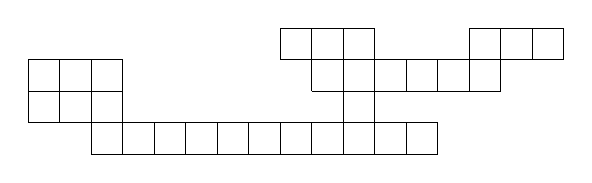
\begin{tikzpicture}[scale=0.4pt]
        \def\a{-5.5}
        \def\b{10.5}

        \draw[color = black!100] (0, 2) -- (3, 2);
        \draw[color = black!100] (0, 3) -- (3, 3);

        \foreach \x in {0, ..., 3} {
            \draw[color = black!100] (\x, 2) -- (\x, 2+1);
        }

        \draw[color = black!100] (0, 3) -- (3, 3);
        \draw[color = black!100] (0, 4) -- (3, 4);

        \foreach \x in {0, ..., 3} {
            \draw[color = black!100] (\x, 3) -- (\x, 3+1);
        }

        \draw[color = black!100] (2, 1) -- (13, 1);
        \draw[color = black!100] (2, 2) -- (13, 2);

        \foreach \x in {2, ..., 13} {
            \draw[color = black!100] (\x, 1) -- (\x, 1+1);
        }

        \draw[color = black!100] (10, 2) -- (11, 2);
        \draw[color = black!100] (10, 3) -- (11, 3);

        \foreach \x in {10, 11} {
            \draw[color = black!100] (\x, 2) -- (\x, 2+1);
        }

        \draw[color = black!100] (9, 3) -- (15, 3);
        \draw[color = black!100] (9, 4) -- (15, 4);

         \foreach \x in {9, ..., 15} {
            \draw[color = black!100] (\x, 3) -- (\x, 3+1);
        }

        \draw[color = black!100] (14, 4) -- (17, 4);
        \draw[color = black!100] (14, 5) -- (17, 5);

         \foreach \x in {14, ..., 17} {
            \draw[color = black!100] (\x, 4) -- (\x, 4+1);
        }

        \draw[color = black!100] (8, 4) -- (11, 4);
        \draw[color = black!100] (8, 5) -- (11, 5);

         \foreach \x in {8, ..., 11} {
            \draw[color = black!100] (\x, 4) -- (\x, 4+1);
        }
    \end{tikzpicture}
\end{center}